% FORMATTING REQUIREMENTS:
% Titular frame
% Introductory frame
% Goals and objectives frame
% C++17 implementation
% Vectorization (AVX)
% Parallelization (std::threads/OpenMP)
% Conclusion frame
% Materials frame
% 
% FONT REQUIREMENTS:
% Serif fonts (Georgia, Palatino, Times New Roman)
% Size title - [24pt ... 54pt] text - [18pt ... 36pt]
% Bold, Italic - semantic highlights
% No more than 3 font types

\documentclass[presentation,18pt]{beamer}

\usepackage[utf8]{inputenc}
\usepackage[T1,T2A]{fontenc}
\usepackage[english,russian]{babel}
\usepackage{amsmath,amsfonts,amssymb}
\usepackage{geometry}

% Set serif font
\renewcommand{\familydefault}{\sfdefault}

\usetheme{Madrid}
\usecolortheme{whale}

\begin{document}

\title[Оптимизация LRnLA]{Оптимизация решения систем дифференциальных уравнений 
	на двумерной сетке с использованием явных численных схем}
\subtitle{LXIII конференция МФТИ}
\author[Ельчинов]{Ельчинов Е. С.\inst{1} \and
									Кудринский А. М.\inst{2}}
\institute[МФТИ]{МФТИ (ГУ) \\
	\vspace{1ex}
	Научный руководитель~--- Хохлов Н. И., к.ф.-м.н., с.н.с., зам. зав. лаб. \\
	(Лаборатория прикладной вычислительной геофизики МФТИ)
	\vspace{1ex}
}
\date{\today}

% Titular frame
\begin{frame}
	\label{titular}
	\titlepage
\end{frame}

% Introductory frame
\begin{frame}[fragile,t]
	\label{introductory}
	\frametitle{Постановка проблемы и актуальность}

	% \begin{block}{Проблема}
	%	Оптимизация моделирования волнового процесса на двумерной сетке
	% \end{block}

	\begin{columns}

	\column{0.65\textwidth}
		\begin{block}{}
			% $U^{n+1} = f\left(U^n, dx, dy, dt\right)$
			\begin{verbatim}
			for (n = 0; n <= MAX_TIME; ++n) {
			  for (X = 0; X <= MAX_X; ++X) {
			    for (Y = 0; Y <= MAY_Y; ++Y) {
			      ...
			      U[n+1] = f(U[n], U[n-1], dx, dy);
			    }
			  }
			  U[n] = U[n+1];
			}
			\end{verbatim}
		\end{block}

	\column{0.30\textwidth}
		\begin{block}{Локальный шаблон}
			% TODO: уточнить параметры!!!
			\begin{figure}
				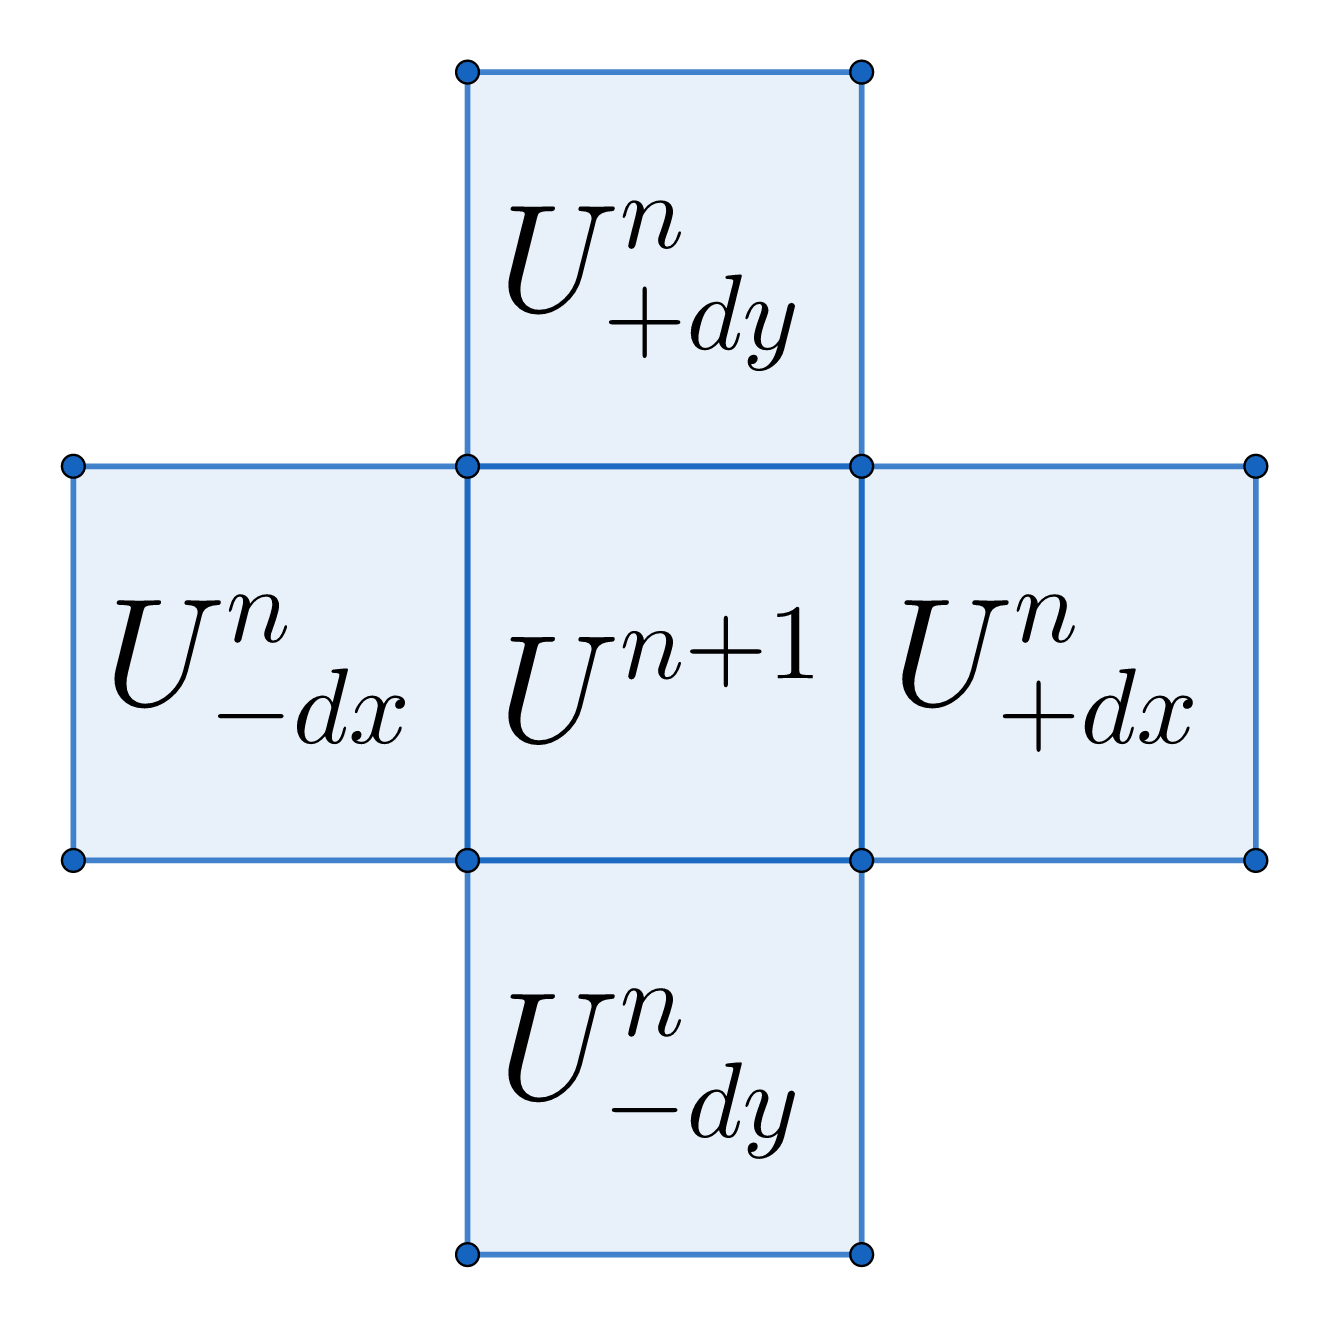
\includegraphics[width=\textwidth]{img/CropStencil.png}
			\end{figure}
		\end{block}

	\end{columns}

	\begin{alertblock}{Характерные параметры}
		\begin{columns}
		\column{0.25\textwidth}
			$\sim 1\,000\,000\,000$ \\ узлов сетки

		\column{0.3\textwidth}
			$\sim 1\,000\,000$ \\ временн\'{ы}х слоев

		\column{0.35\textwidth}
			$\sim 1\,000$ \\ задач моделирования
		\end{columns}
	\end{alertblock}

\end{frame}

% TODO
% Goals & objectives frame
\begin{frame}[t]
	\label{goals}
	\frametitle{Цели и задачи}

	\begin{block}{Цель}
		Использование современного C++, возможностей современных процессоров и 
		кэша в оптимизации цикла вычислений.
	\end{block}

	\begin{columns}

	\column{0.4\textwidth}
		\begin{block}{CPU}
			\begin{itemize}
				\item AVX
				\item 4, 6, 8, 10\ldots ядер
				\item потоки внутри ядра
				\item L1, L2, L3 кэши
				\item предвыборка команд
			\end{itemize}
		\end{block}

	\column{0.4\textwidth}
		\begin{block}{C++}
			\begin{itemize}
				\item шаблоны
				\item constexpr~-- функции
				\item if constexpr
				\item Thread support library
				\item интеграция с OpenMP
			\end{itemize}
		\end{block}

	\end{columns}
\end{frame}

% Tiling algorithms
\begin{frame}[t]
	\label{tiling}
	\frametitle{Алгоритмы тайлинга}

	\begin{columns}

	\column{0.4\textwidth}
		\begin{block}{ConeFold}
			\begin{figure}
				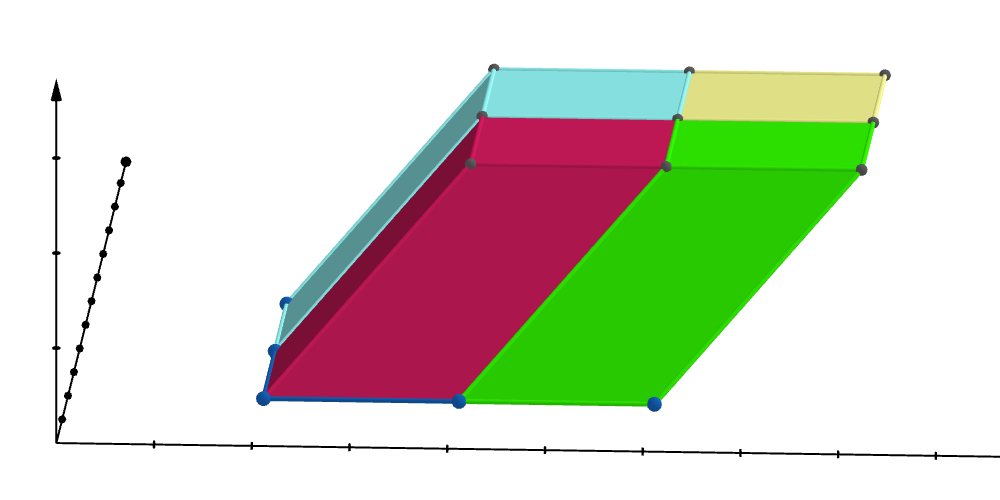
\includegraphics[width=\textwidth]{img/CropConeFold.png}
			\end{figure}
		\end{block}

		\begin{block}{DiamondTorre}
			\begin{figure}
				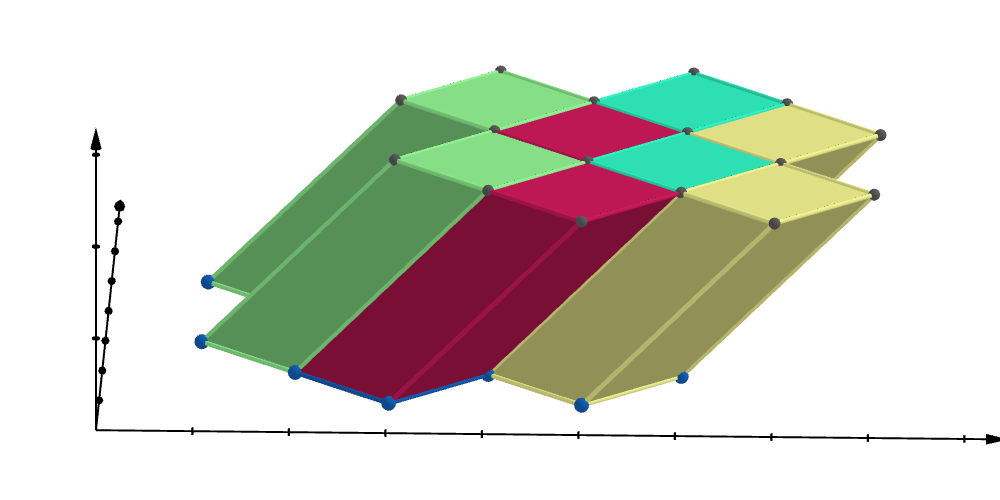
\includegraphics[width=\textwidth]{img/CropDiamondTorre.png}
			\end{figure}
		\end{block}

	\column{0.55\textwidth}
		\begin{alertblock}{Зависимость времени работы от размера сетки}
			\begin{figure}
				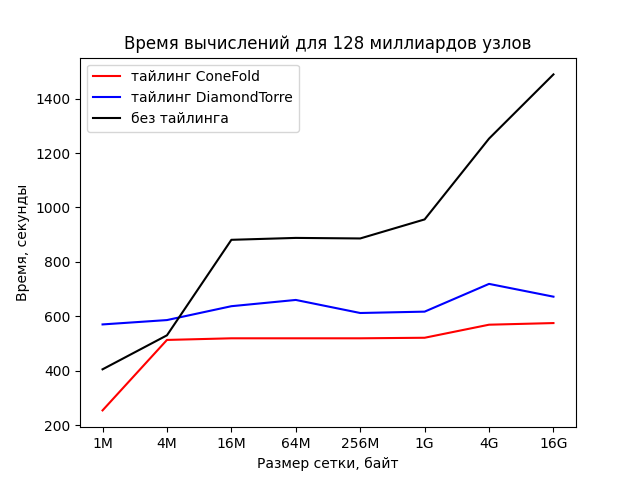
\includegraphics[width=\textwidth]{img/GraphTiling.png}
			\end{figure}
		\end{alertblock}

	\end{columns}
\end{frame}

% Vectorization
\begin{frame}[t]
	\label{vectorization}
	\frametitle{Векторизация}

	\begin{columns}

	\column{0.4\textwidth}
		\begin{block}{AVX, шаблон $2 \times 2$}
			\begin{figure}
				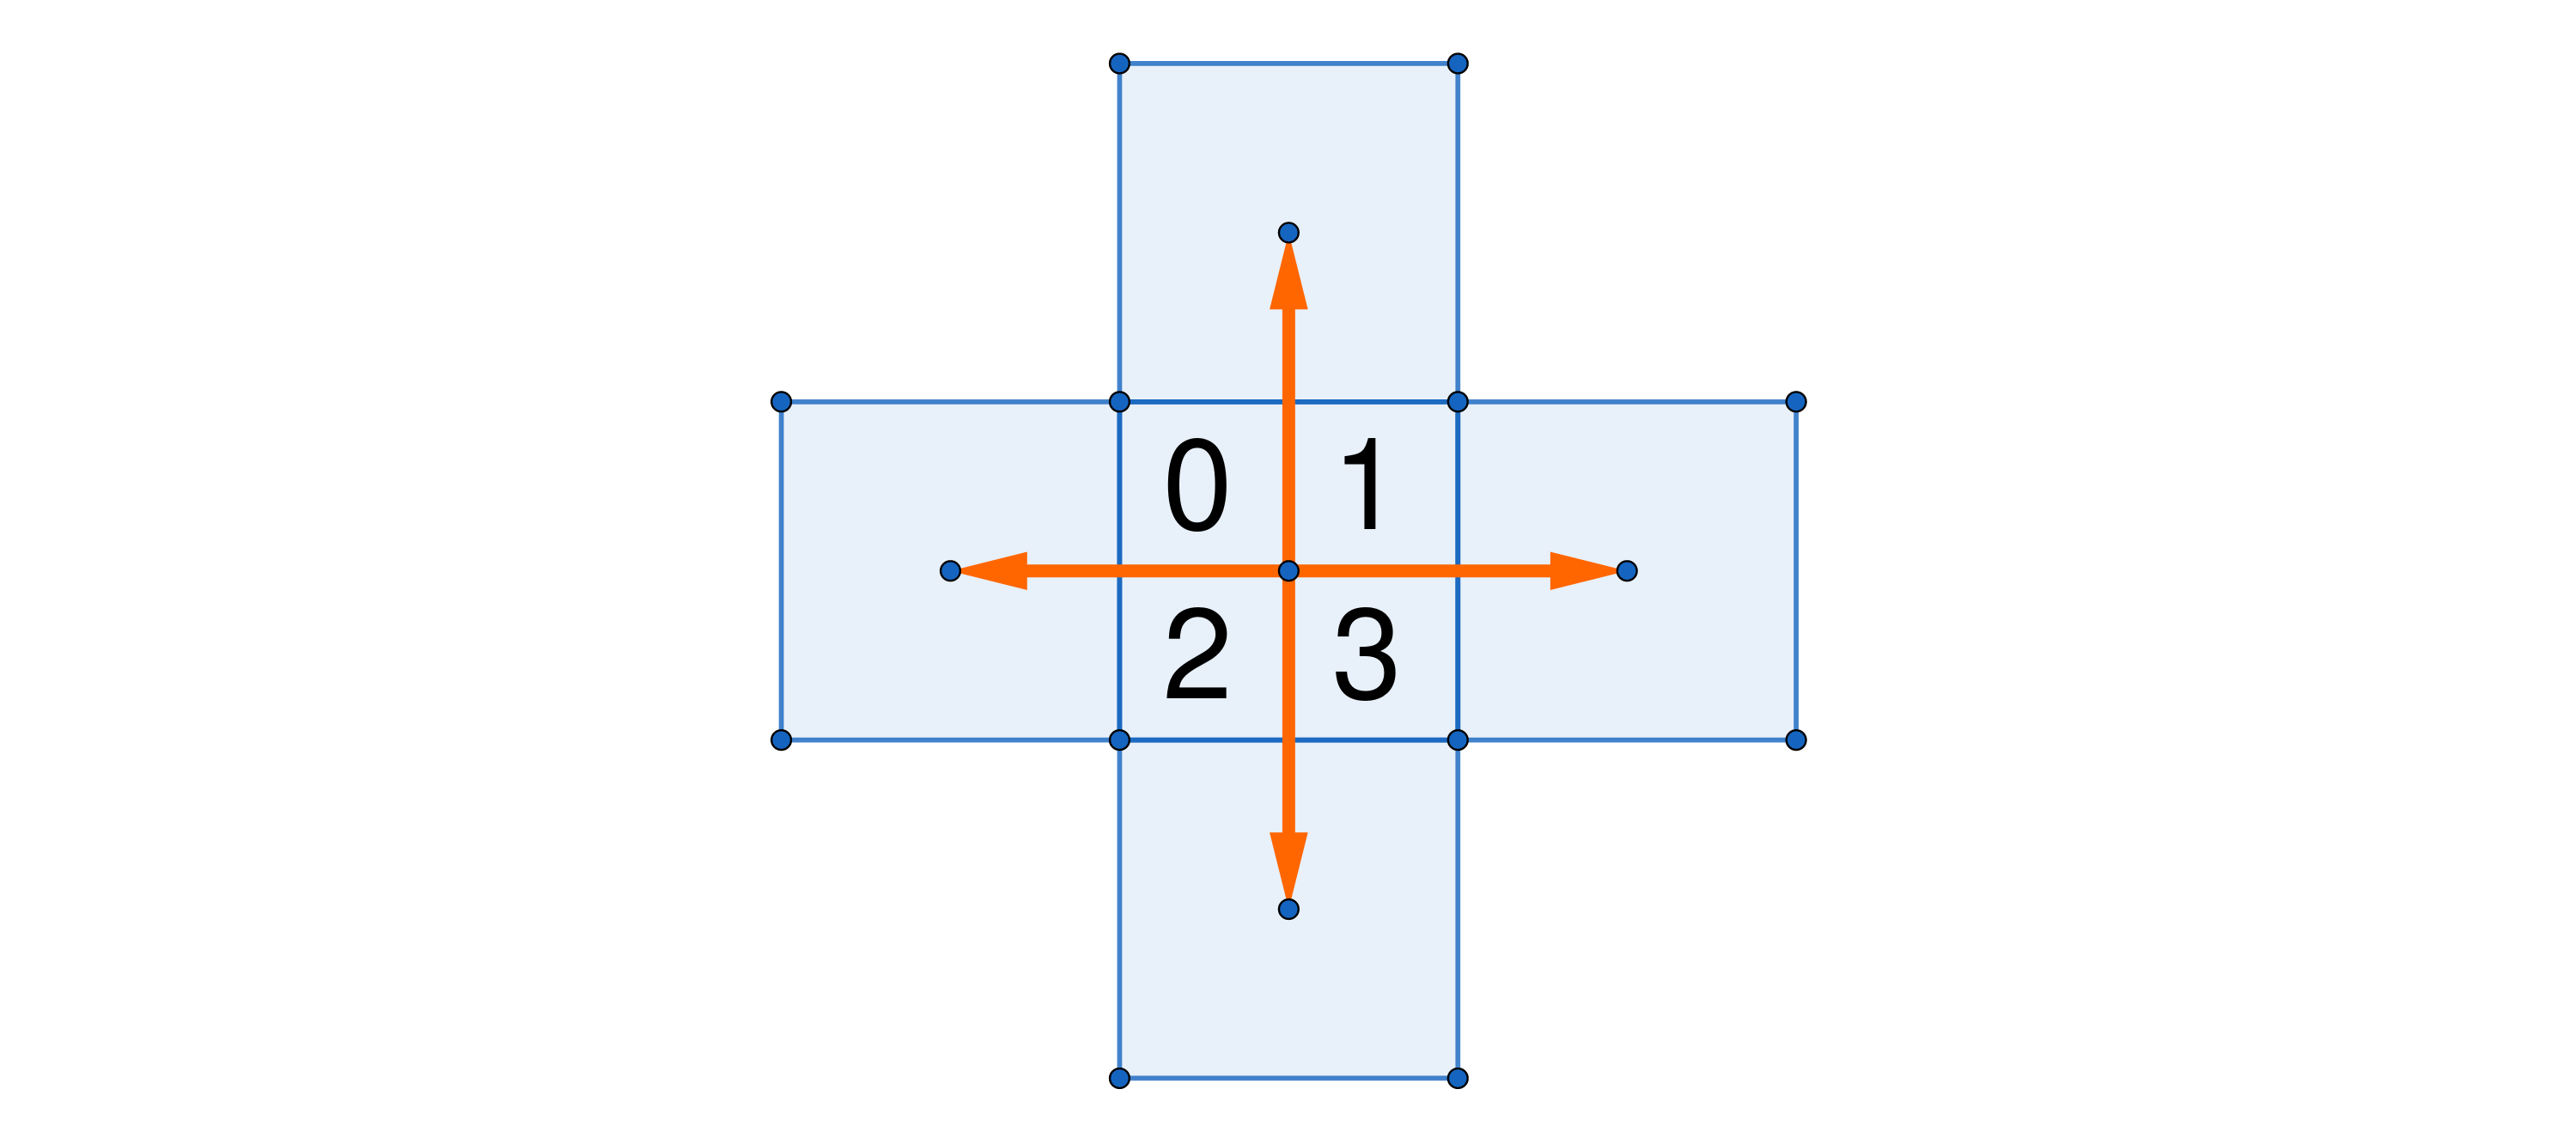
\includegraphics[width=\textwidth]{img/CropAVX2x2.png}
			\end{figure}
		\end{block}

		\begin{block}{AVX, шаблон $1 \times 4$}
			\begin{figure}
				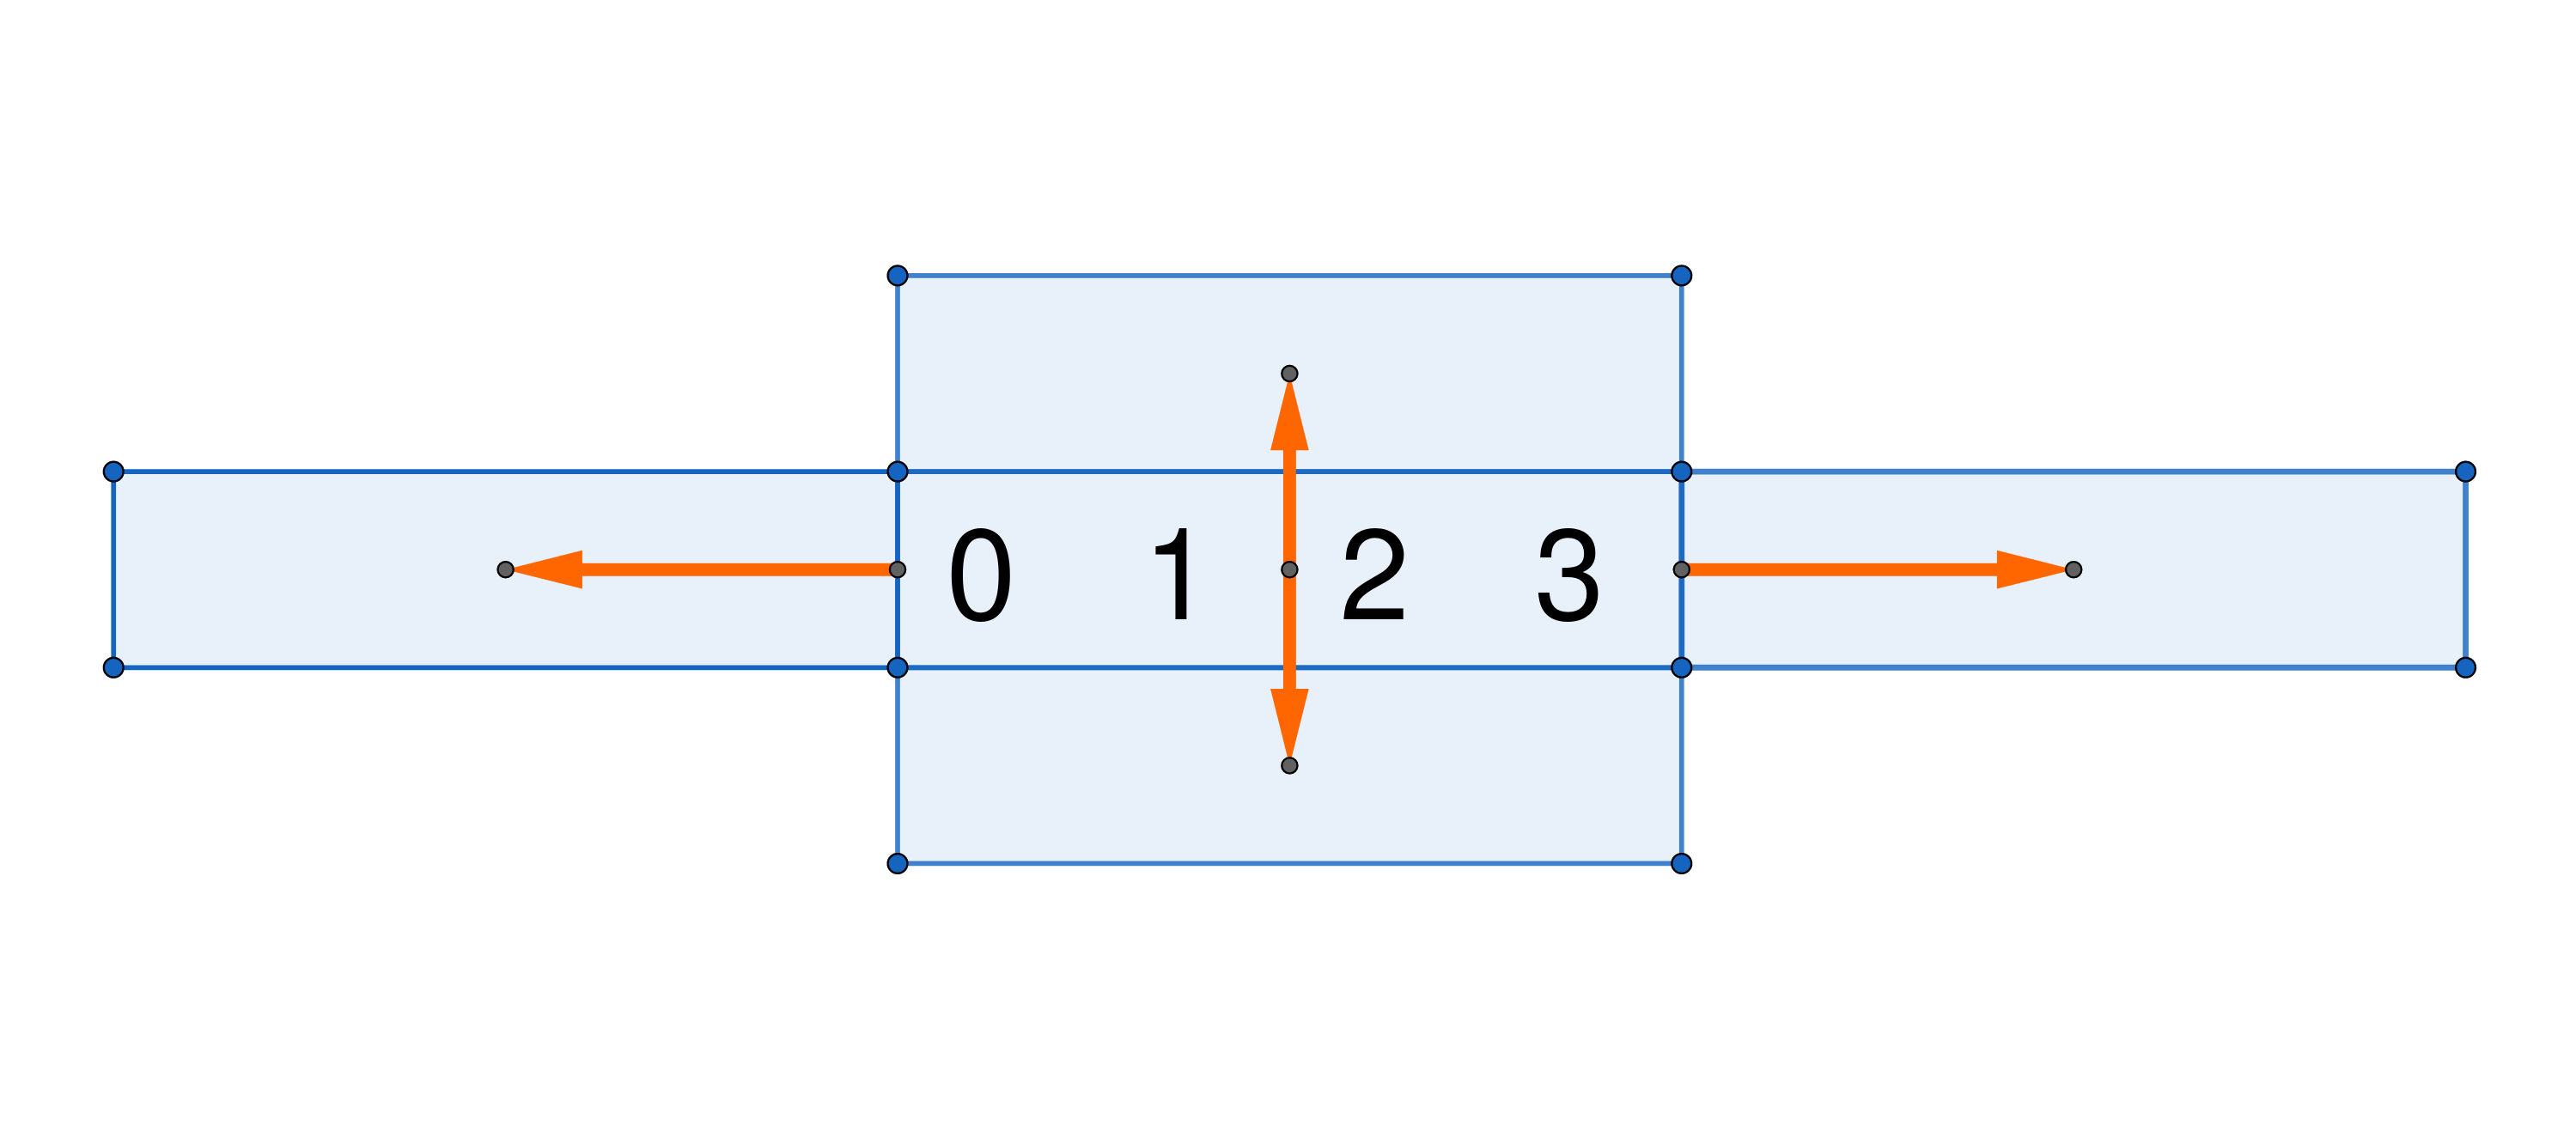
\includegraphics[width=\textwidth]{img/CropAVX1x4.png}
			\end{figure}
		\end{block}

	\column{0.55\textwidth}
		\begin{alertblock}{Зависимость времени работы от размера сетки}
			\begin{figure}
				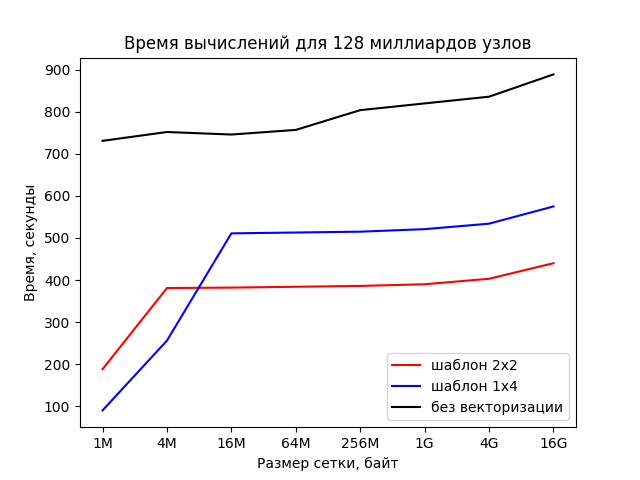
\includegraphics[width=\textwidth]{img/GraphVector.png}
			\end{figure}
		\end{alertblock}

	\end{columns}
\end{frame}

% Data order
\begin{frame}[t]
	\label{data-order}
	\frametitle{Способы хранения данных}

	\begin{columns}

	\column{0.5\textwidth}
		\begin{block}{Линейный порядок}
			\begin{itemize}
				\item Простые расчеты
				\item Невысокая локальность
			\end{itemize}
		\end{block}

		\begin{alertblock}{} % Зависимость времени работы от размера сетки
			\begin{figure}
				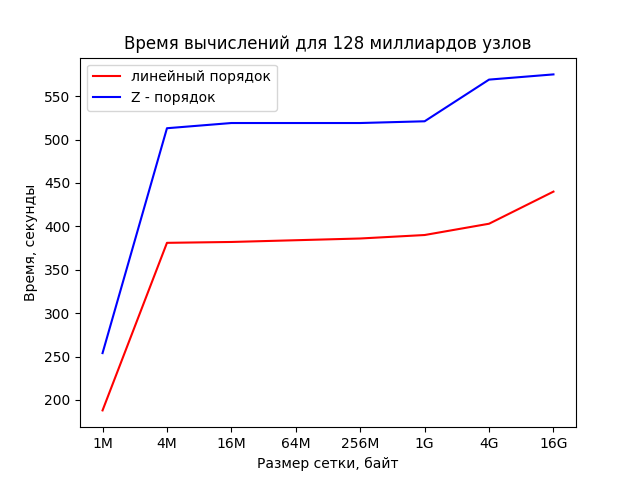
\includegraphics[width=\textwidth]{img/GraphLayout.png}
			\end{figure}
		\end{alertblock}

	\column{0.4\textwidth}
		\begin{block}{Z~-- порядок}
			\begin{itemize}
				\item Более сложные расчеты
				\item Высокая локальность
			\end{itemize}

			\begin{figure}
				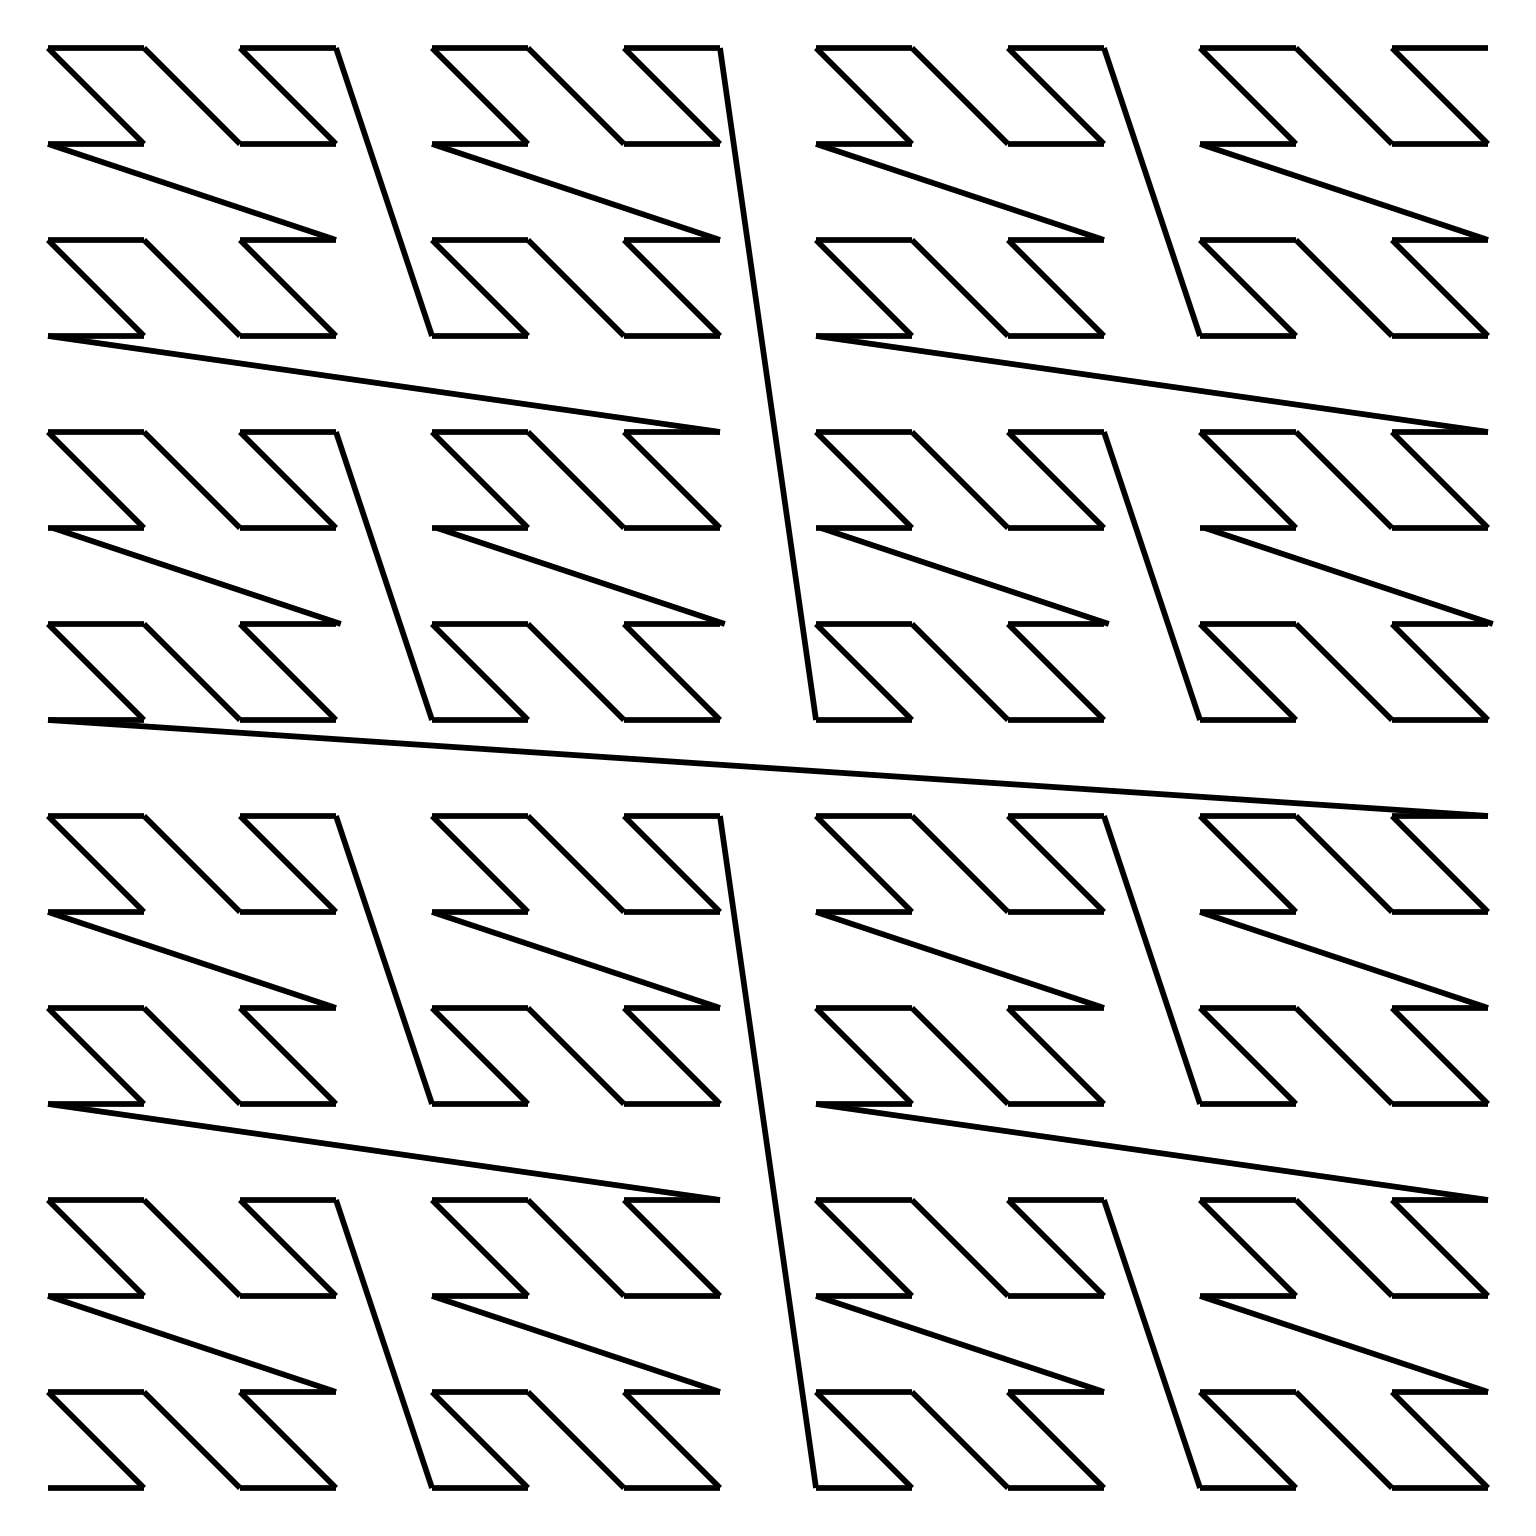
\includegraphics[width=\textwidth]{img/ZOrderCurve.png}
			\end{figure}
		\end{block}

	\end{columns}
\end{frame}

% Conclusion frame
\begin{frame}
	\label{conclusion}
	\frametitle{Результаты}
	\framesubtitle{Зависимость времени работы от размера сетки}

	\begin{columns}

	\column{0.1\textwidth}

	\column{0.75\textwidth}
		\begin{block}{}
			\begin{figure}
				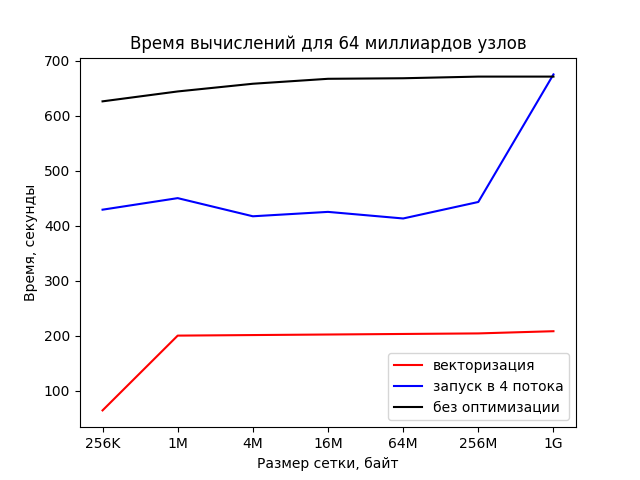
\includegraphics[width=\textwidth]{img/GraphFinal.png}
			\end{figure}
		\end{block}

	\column{0.1\textwidth}

	\end{columns}
\end{frame}

% Materials frame
\begin{frame}
	\label{materials}
	\frametitle{Материалы}
\end{frame}

\end{document}
